\documentclass{ieeeaccess}
\usepackage{cite}
\usepackage{amsmath,amssymb,amsfonts}
\usepackage{algorithmic}
\usepackage{algorithm}
\usepackage{graphicx}
\usepackage{textcomp}
\usepackage{booktabs}
\usepackage{url}
\usepackage{amsthm}
\newtheorem{definition}{Definition}
\newtheorem{remark}{Remark}
% AUTO-GENERATED by eval/aggregate.py -- do not edit
\newcommand{\nTasks}{1{,}000}
\newcommand{\nBird}{500}
\newcommand{\nSpider}{500}
\newcommand{\nSpiderValid}{881}
\newcommand{\nBirdChallenging}{460}
\newcommand{\nNonPermitted}{200}
\newcommand{\permRateFull}{100.0}
\newcommand{\permRateRestricted}{44.5}
\newcommand{\permRatePartition}{52.4}
\newcommand{\exHaikuBzero}{65.8}
\newcommand{\exHaikuBone}{47.0}
\newcommand{\exHaikuBthree}{54.5}
\newcommand{\wreqHaiku}{23.4}
\newcommand{\wappHaiku}{22.2}
\newcommand{\exAfterWidHaiku}{47.7}
\newcommand{\exHaikuTse}{59.3}
\newcommand{\dExHaikuBone}{-18.8}
\newcommand{\dExLoHaikuBone}{-22.0}
\newcommand{\dExHiHaikuBone}{-15.5}
\newcommand{\dExHaikuBoneBird}{-21.0}
\newcommand{\dExHaikuBoneSpider}{-16.6}
\newcommand{\dExHaikuBthree}{-11.3}
\newcommand{\dExLoHaikuBthree}{-14.4}
\newcommand{\dExHiHaikuBthree}{-8.2}
\newcommand{\dExHaikuBthreeBird}{-21.0}
\newcommand{\dExHaikuBthreeSpider}{-1.6}
\newcommand{\dExHaikuTse}{-6.5}
\newcommand{\dExLoHaikuTse}{-9.6}
\newcommand{\dExHiHaikuTse}{-3.5}
\newcommand{\dExHaikuTseBird}{-16.8}
\newcommand{\dExHaikuTseSpider}{3.8}
\newcommand{\exSonnetBzero}{83.5}
\newcommand{\exSonnetBthree}{64.3}
\newcommand{\wreqSonnet}{24.5}
\newcommand{\wappSonnet}{23.7}
\newcommand{\exAfterWidSonnet}{67.1}
\newcommand{\exSonnetTse}{72.2}
\newcommand{\dExSonnetBthree}{-19.2}
\newcommand{\dExLoSonnetBthree}{-22.2}
\newcommand{\dExHiSonnetBthree}{-16.3}
\newcommand{\dExSonnetBthreeBird}{-33.2}
\newcommand{\dExSonnetBthreeSpider}{-5.2}
\newcommand{\dExSonnetTse}{-11.3}
\newcommand{\dExLoSonnetTse}{-13.9}
\newcommand{\dExHiSonnetTse}{-8.7}
\newcommand{\dExSonnetTseBird}{-19.0}
\newcommand{\dExSonnetTseSpider}{-3.6}
\newcommand{\nEtwoRuns}{7000}
\newcommand{\nRunsPerCondHaiku}{1000}
\newcommand{\nRunsPerCondSonnet}{1000}
\newcommand{\npRefuseBzero}{59.5}
\newcommand{\npSilentBzero}{40.5}
\newcommand{\npRefuseTse}{58.0}
\newcommand{\npSilentTse}{40.0}
\newcommand{\npExceedReq}{121}
\newcommand{\medCompile}{8.4}
\newcommand{\pNinetyFiveCompile}{22.1}
\newcommand{\medTeardown}{4.3}
\newcommand{\pNinetyFiveTeardown}{13.6}
\newcommand{\medQueryBzero}{0.9}
\newcommand{\pNinetyFiveQueryBzero}{98.8}
\newcommand{\medQueryTse}{0.9}
\newcommand{\pNinetyFiveQueryTse}{151.0}
\newcommand{\medQueryRatio}{1.11}
\newcommand{\medObjects}{5}
\newcommand{\eFourErrors}{38}
\newcommand{\eFourEqual}{960}
\newcommand{\eFourOk}{962}
\newcommand{\eFourGroupingErr}{35}
\newcommand{\eFourTimeout}{2}
\newcommand{\medInferS}{8.1}
\newcommand{\pNinetyFiveInferS}{22.5}
\newcommand{\bypassAttempts}{928}
\newcommand{\bypassSuccess}{0}
\newcommand{\bypassTypes}{32}
\newcommand{\bypassDbs}{29}
\newcommand{\exfHaikuCtxBzero}{89.0}
\newcommand{\obtHaikuCtxBzero}{90.5}
\newcommand{\exfHaikuCtxBtwo}{90.0}
\newcommand{\obtHaikuCtxBtwo}{91.0}
\newcommand{\exfHaikuCtxBthree}{84.0}
\newcommand{\obtHaikuCtxBthree}{85.5}
\newcommand{\exfHaikuCtxTse}{25.0}
\newcommand{\obtHaikuCtxTse}{25.5}
\newcommand{\tseLeaksHaikuCtx}{49}
\newcommand{\tseLeaksInitHaikuCtx}{5}
\newcommand{\tseLeaksWidenHaikuCtx}{45}
\newcommand{\exfSonnetCtxBzero}{91.0}
\newcommand{\obtSonnetCtxBzero}{91.0}
\newcommand{\exfSonnetCtxBtwo}{89.5}
\newcommand{\obtSonnetCtxBtwo}{91.0}
\newcommand{\exfSonnetCtxBthree}{83.0}
\newcommand{\obtSonnetCtxBthree}{86.5}
\newcommand{\exfSonnetCtxTse}{27.6}
\newcommand{\obtSonnetCtxTse}{30.1}
\newcommand{\tseLeaksSonnetCtx}{54}
\newcommand{\tseLeaksInitSonnetCtx}{6}
\newcommand{\tseLeaksWidenSonnetCtx}{49}
\newcommand{\exfHaikuDbBzero}{0.0}
\newcommand{\obtHaikuDbBzero}{0.5}
\newcommand{\exfHaikuDbBthree}{0.0}
\newcommand{\obtHaikuDbBthree}{0.0}
\newcommand{\exfHaikuDbTse}{0.0}
\newcommand{\obtHaikuDbTse}{0.0}
\newcommand{\eFiveMaxPHolm}{4.1e-27}
\newcommand{\dbSeenBzero}{41.9}
\newcommand{\dbSeenBthree}{33.8}
\newcommand{\dbSeenTse}{30.3}
\newcommand{\dbSeenN}{210}
\newcommand{\dbSeenAttempted}{12}
\newcommand{\dbN}{594}
\newcommand{\exfHaikuCtxDeny}{2.6}
\newcommand{\exfHaikuCtxDenyLo}{0.5}
\newcommand{\exfHaikuCtxDenyHi}{5.2}
\newcommand{\obtHaikuCtxDeny}{2.6}
\newcommand{\denyLeaksHaiku}{5}
\newcommand{\denyLeaksInScopeHaiku}{5}
\newcommand{\pDenyHaiku}{5.1e-12}
\newcommand{\exfSonnetCtxDeny}{2.6}
\newcommand{\exfSonnetCtxDenyLo}{0.5}
\newcommand{\exfSonnetCtxDenyHi}{5.2}
\newcommand{\obtSonnetCtxDeny}{2.6}
\newcommand{\denyLeaksSonnet}{5}
\newcommand{\denyLeaksInScopeSonnet}{5}
\newcommand{\pDenySonnet}{7.1e-15}
\newcommand{\ablExKzero}{50.5}
\newcommand{\ablDKzero}{-9.0}
\newcommand{\ablDLoKzero}{-15.0}
\newcommand{\ablDHiKzero}{-3.0}
\newcommand{\ablWreqKzero}{26.5}
\newcommand{\ablExKtwo}{65.5}
\newcommand{\ablDKtwo}{6.0}
\newcommand{\ablDLoKtwo}{-0.5}
\newcommand{\ablDHiKtwo}{12.5}
\newcommand{\ablWreqKtwo}{1.5}
\newcommand{\ablExStrict}{58.5}
\newcommand{\ablDStrict}{-1.0}
\newcommand{\ablDLoStrict}{-7.0}
\newcommand{\ablDHiStrict}{5.0}
\newcommand{\ablWreqStrict}{19.0}
\newcommand{\ablExDeny}{51.5}
\newcommand{\ablDDeny}{-8.0}
\newcommand{\ablDLoDeny}{-14.5}
\newcommand{\ablDHiDeny}{-1.5}
\newcommand{\ablWreqDeny}{19.0}
\newcommand{\ablN}{200}
\newcommand{\ablExDefault}{59.5}
\newcommand{\ablExBzero}{67.5}
\newcommand{\seedReps}{3}
\newcommand{\seedSubsetN}{100}
\newcommand{\seedDiffMin}{-6.0}
\newcommand{\seedDiffMax}{0.0}
\newcommand{\seedExBzeroMin}{65.0}
\newcommand{\seedExBzeroMax}{67.0}
\newcommand{\seedExTseMin}{61.0}
\newcommand{\seedExTseMax}{65.0}
\newcommand{\widNAuto}{368}
\newcommand{\widCanaryReqAuto}{82.6}
\newcommand{\widCanaryGrantedAuto}{74.5}
\newcommand{\widExfilAuto}{64.1}
\newcommand{\widRejectedExceedAuto}{32}
\newcommand{\widNStrict}{375}
\newcommand{\widCanaryReqStrict}{83.7}
\newcommand{\widCanaryGrantedStrict}{64.3}
\newcommand{\widExfilStrict}{55.5}
\newcommand{\widRejectedExceedStrict}{30}
\newcommand{\widGrantedOutsideE}{0}
\newcommand{\widGrantedTotal}{586}
\newcommand{\apiSpend}{57.94}


% Review version: remove journal identifiers (volume/year footer, DOI line). The editorial office adds them later.
\usepackage{etoolbox}
\makeatletter
\patchcmd{\ps@headings}{VOLUME\ \thevol, \theyear}{}{}{}
\patchcmd{\ps@headings}{VOLUME\ \thevol, \theyear}{}{}{}
\patchcmd{\ps@titlepage}{VOLUME\ \thevol, \theyear}{}{}{}
\patchcmd{\ps@titlepage}{VOLUME\ \thevol, \theyear}{}{}{}
\pagestyle{headings}
\doi{}
\def\doifont#1\@doi{}
\makeatother
\newcommand{\artifacturl}{\url{https://github.com/sangaraju1988/task-scoped-entitlements}}
\begin{document}

\title{Task-Scoped Data Entitlements: Deriving and Database-Enforcing Least-Privilege Data Access for LLM Agents}
\author{\uppercase{Venkata M Sangaraju}\authorrefmark{1}}
\address[1]{Independent Researcher, Leander, TX 78641 USA (e-mail: sangaraju1988@gmail.com)}
\tfootnote{This work received no external funding.}

\markboth
{Sangaraju: Task-Scoped Data Entitlements for LLM Agents}
{Sangaraju: Task-Scoped Data Entitlements for LLM Agents}

\corresp{Corresponding author: Venkata M Sangaraju (e-mail: sangaraju1988@gmail.com).}

\begin{abstract}
LLM data agents usually query databases with their user's full entitlement, and tool-level least privilege does not
narrow which rows and columns an allowed query tool can reach. We present task-scoped entitlements (TSE): a trusted
broker infers the tables, columns and rows a natural-language task needs, compiles that scope into an ephemeral
PostgreSQL role and security-barrier views owned by the user's role, and offers a bounded, audited widening request
when the scope is insufficient. In a preregistered evaluation on \nTasks{} BIRD and Spider tasks with Claude Haiku~5.5,
Claude Sonnet~5.5 and open-weight agents, under synthetic role policies, TSE scopes exposed \oerColReduction-fold
fewer columns and \oerCellReduction-fold fewer cells than the full entitlement (\oerCellReductionSuff-fold where the
scope sufficed). Execution accuracy changed by \dExHaikuTse{} (Haiku) and \dExSonnetTse{} (Sonnet) percentage points;
with a stronger broker model, by \hbDHaiku{} and \hbDSonnet{} (exploratory). Under injection naming an out-of-task
column, exfiltration fell from \exfSonnetCtxBzero\% to \exfSonnetCtxTse\% (Sonnet). An injection that made the agent
request the column succeeded in \widExfilAutoSonnet\% of runs under automatic approval, but in
\widExfilJudgeSonnet\% when a broker-side judge that sees only the original task approved widening (exploratory).
Scripted bypass attempts succeeded in \bypassSuccess{} of \bypassAttempts{} cases, while a SQL-parsing gate
enforcing the same scope admitted queries hidden in function arguments. TSE rests on scope-inference quality (sufficient for \suffTse\% of tasks) and correct database
enforcement; it does not protect against inference from in-scope data, covert channels, misuse of in-scope data, or
malicious users.
\end{abstract}


\begin{keywords}
Access control, database security, large language models, least privilege, LLM agents, prompt injection,
row-level security, text-to-SQL.
\end{keywords}

\titlepgskip=-21pt
\maketitle

\section{Introduction}
\label{sec:introduction}

\PARstart{L}{arge} language model (LLM) agents increasingly answer analytics questions by writing and running SQL on
a user's behalf. Such an agent usually connects with the user's own credential, so it can read everything the user
can read. Consider an analyst at a school district who asks an agent: \emph{``How many charter schools in Alameda
County offer a free-meal program?''} The answer needs three columns of two tables and the rows of one county. The
analyst's entitlement, however, covers every school, every test score and every contact field in the database. If the
agent processes untrusted content, for example a note in a retrieved document or a text value stored in the
database, an injected instruction can make it read and repeat data the question never needed~\cite{greshake2023not,debenedetti2024agentdojo}.
The agent acts as a confused deputy~\cite{hardy1988confused}: it holds the user's authority for one narrow purpose but
can be steered to use all of it.

Least privilege says a subject should run with only the privileges its job needs~\cite{saltzer1975protection,dennis1966programming,nist80053r5}.
For agents, recent systems apply this to \emph{tools}: they decide per task which tools, and sometimes which tool
arguments, are allowed~\cite{zhu2025miniscope,shi2025progent,cai2025agentsentry,zhu2026igac,zheng2026intentcap,ruan2024toolemu}.
For a data agent, however, the relevant tool is typically a single \texttt{run\_query} interface. Once it is allowed,
the data the agent can reach is unchanged: still the full entitlement. Databases have long supported finer control
through views, column grants and row-level security~\cite{stonebraker1975query,rizvi2004extending,pgrls,oraclevpd},
and access-controlled text-to-SQL systems enforce a \emph{user's} policy~\cite{fei2026rbac,klisura2026role,miyamoto2026pccsql,kim2026securemcp}.
Practitioners write static scoped views per role. None of these narrows the data an agent can reach to what the
\emph{current task} needs.

We propose \emph{task-scoped entitlements} (TSE). Before an agent starts, a trusted broker infers a relational scope
from the natural-language task: which tables, columns and rows it needs. The broker compiles that scope into an
ephemeral PostgreSQL role and \texttt{security\_barrier} views that are owned by the user's role, hands the agent a
login for that role as its only credential, and drops everything when the task ends. Because the views are owned by
the user's role, the database bounds them by the user's entitlement even when the inference is wrong. When the
inferred scope is insufficient, the agent can file a structured widening request, which is bounded by the
entitlement, decided by a policy, and logged.

\subsection{Contributions}
\begin{itemize}
\item[\textbf{C1}] A formal model of task scopes: entitlement, task scope, needed data, sufficiency, minimality, a
column/row/cell over-exposure ratio (OER), and a widening bound, with a design guarantee stated under explicit trust
assumptions (Section~\ref{sec:model}).
\item[\textbf{C2}] A scope-inference procedure that combines an LLM proposal with an automatically built semantic
layer, deterministic schema linking, grounding of row filters in the task text, foreign-key closure, and a
conservativeness parameter $k$ (Section~\ref{sec:inference}).
\item[\textbf{C3}] Database enforcement independent of the model: compilation to ephemeral roles and
\texttt{security\_barrier} views owned by the user role, with idempotent teardown (Section~\ref{sec:enforcement}).
\item[\textbf{C4}] A controlled widening protocol that turns inference errors into bounded, auditable requests
(Section~\ref{sec:widening}).
\item[\textbf{C5}] A preregistered evaluation on \nTasks{} public text-to-SQL tasks (BIRD and Spider) with frontier
and open-weight agents in two agent frameworks, four baselines, indirect prompt injection, widening abuse, and
\bypassAttempts{} enforcement-bypass attempts (Sections~\ref{sec:setup}--\ref{sec:results}).
\end{itemize}

\subsection{Summary of findings}
Under synthetic-policy entitlements, the default TSE scope reduces the columns an agent can reach by a factor of
\oerColReduction{} (geometric mean) and the reachable cells by a factor of \oerCellReduction{} relative to the full
entitlement. The scope is sufficient for the gold query on \suffTse\% of tasks; this inference quality is the
load-bearing assumption of the approach, and we quantify it directly. With widening, execution accuracy changed by
\dExHaikuTse{} percentage points for Claude Haiku~5.5 (95\% CI [\dExLoHaikuTse, \dExHiHaikuTse]) and by
\dExSonnetTse{} points for Claude Sonnet~5.5 (95\% CI [\dExLoSonnetTse, \dExHiSonnetTse]) relative to full access, a smaller loss than static role views (\dExHaikuBone{} points) or prompt-level schema
pruning with full credentials (\dExHaikuBthree{} points) for Haiku~5.5. A more conservative scope ($k{=}2$) brought
accuracy to \ablExKtwo\% against \ablExBzero\% for B0 on an exploratory subset.
Under indirect prompt injection that targets out-of-task data, exfiltration fell from \exfSonnetCtxBzero\% (B0) to
\exfSonnetCtxTse\% (TSE) for Sonnet~5.5 and from \exfHaikuCtxBzero\% to \exfHaikuCtxTse\% for Haiku~5.5; nearly all remaining leaks used
approved widening, and with widening denied exfiltration was \exfSonnetCtxDeny\% and \exfHaikuCtxDeny\%. None of
our \bypassAttempts{} scripted bypass attempts reached out-of-scope data. Provisioning takes \medCompile{}\,ms
(median) and teardown \medTeardown{}\,ms.

\subsection{What we do not claim}
TSE reduces the data reachable for a task; it does not prevent all leakage. It does not protect against inference or
aggregation over data inside the scope, covert or timing channels, exfiltration of in-scope data, a malicious
authorized user, or a compromised broker, and table and column names remain visible in the catalog. Its benefit
depends on two assumptions that can fail: the quality of scope inference (too narrow causes failures or widening;
too broad reduces the benefit) and the correctness of database enforcement. Views, row-level security and query
modification are established techniques that we use unchanged; the new parts are listed in
Section~\ref{sec:whatsnew}. We make no claim about production readiness: the schemas are public benchmarks and the
entitlements are synthetic.

The rest of the paper is organized as follows. Section~\ref{sec:threat} states the threat model,
Section~\ref{sec:related} positions the work, Sections~\ref{sec:model}--\ref{sec:enforcement} present the model and
system, Sections~\ref{sec:setup}--\ref{sec:results} the evaluation, and Sections~\ref{sec:discussion}--\ref{sec:conclusion}
discuss threats, limitations and future work.

\section{Background and Threat Model}
\label{sec:threat}

\subsection{Setting}
A user $u$ delegates an analytics task, stated in natural language, to an LLM agent. The agent answers by issuing
SQL through a query tool. Without our mechanism, the agent's database credential carries $u$'s full
entitlement $E(u)$ (condition B0 in our evaluation): it can read every column and row $u$ can read, regardless of
what the task needs. The trusted broker that provisions the agent also sees the task text and the schema.

\subsection{Adversary}
The adversary wants the agent to read, and reveal, data that the current task does not need. We consider an
adversary who can:
\begin{enumerate}
\item place instructions in content the agent reads: database text fields returned by queries, and documents or
notes attached to the task context (indirect prompt injection~\cite{greshake2023not});
\item thereby make the agent issue arbitrary SQL on its connection, including attempts to bypass enforcement
(catalog reads, role switching, \texttt{COPY}, leaky functions, error and timing side channels);
\item make the agent file widening requests with plausible reasons;
\item observe the agent's final answer (the exfiltration channel we measure).
\end{enumerate}
The adversary cannot modify the broker, the database configuration or the user's entitlement, and holds no
database credential of its own.

\subsection{Trust assumptions}
We rely on A1--A4 (Section~\ref{sec:assumptions}): the DBMS enforces grants, row policies, view ownership and
\texttt{security\_barrier} correctly; the ephemeral login is the agent's only credential; the broker is trusted;
and no involved role has bypass privileges.

\subsection{In scope and out of scope}
\textbf{In scope:} reducing the data an agent can \emph{reach} for a task, measured as over-exposure; containing
injected requests for out-of-task data; bounding and auditing widening; and robustness of the enforcement
against the bypass attempts listed above.

\textbf{Out of scope (not protected):}
(i)~inference and aggregation attacks that use data inside the task scope or inside $E(u)$~\cite{denning1979tracker,adam1989security};
(ii)~covert and timing channels;
(iii)~exfiltration of data that is inside the task scope (TSE narrows what can leak; it does not stop the agent
from repeating in-scope data);
(iv)~a malicious authorized user, who already holds $E(u)$;
(v)~a compromised broker or a misconfigured entitlement $E(u)$;
(vi)~schema metadata: table and column names are visible in the PostgreSQL catalog to every role.
TSE therefore reduces the data reachable per task; it does not prevent all leakage.

\section{Related Work}
\label{sec:related}

We organize prior work into four groups and then state precisely what this paper adds.
Table~\ref{tab:mechanisms} compares mechanisms as described by their authors; it contains no
performance numbers, because we did not run those systems (Section~\ref{sec:setup} describes the
re-implemented baselines we did run).

\subsection{Fine-grained access control and query modification in databases}
Least privilege is a design principle for protection systems~\cite{saltzer1975protection}.
Relational databases realize it with discretionary grants on tables and
columns~\cite{griffiths1976authorization} and role-based models~\cite{sandhu1996rbac,ferraiolo2001nist},
with attribute-based variants~\cite{hu2014abac}. Row-level restriction has a long history:
Stonebraker's query modification rewrites a user query by conjoining the predicates of the views a
user may see~\cite{stonebraker1975query}; Rizvi et al.\ distinguish the \emph{Truman} model, which
silently rewrites queries to a user's view, from the \emph{non-Truman} model, which accepts a query only
if it is answerable from authorized views~\cite{rizvi2004extending}; Kabra et al.\ show how predicate
pushdown can leak information past such rewrites~\cite{kabra2006redundancy}. Commercial systems expose
these ideas as Oracle Virtual Private Database policies~\cite{oraclevpd} and PostgreSQL row-security
policies and \texttt{security\_barrier} views~\cite{pgrls,pgsecbarrier}. Surveys summarize the
area~\cite{bertino2005database}. Information disclosure through views has been formalized
\cite{miklau2004formal}, and statistical-database work shows that aggregate answers over authorized data
can still reveal individual values~\cite{denning1979tracker,adam1989security}. All of this machinery
enforces a policy written by an administrator for a user or role; none of it derives the policy from a
task description.

\subsection{Purpose-based access and privacy-by-design databases}
Hippocratic databases attach purposes to data and limit disclosure to what a stated purpose
requires~\cite{agrawal2002hippocratic,lefevre2004limiting}; purpose-based access control models purposes
hierarchically and checks access purposes against intended purposes~\cite{byun2008purpose}. Contextual
integrity frames privacy as appropriate information flow for a context~\cite{barth2006contextual}, and
data-minimization requirements appear in regulation~\cite{gdpr2016}. Purposes in these systems are
declared from a fixed vocabulary and bound to stored data in advance. Our task scope is closest in spirit
to a per-request purpose, but it is derived automatically from free-text tasks and expressed directly as a
relational scope (columns, row predicates), not as purpose labels. Two agent systems share this per-task view of
context. Conseca generates a security policy for each task from trusted context and enforces it deterministically on
agent actions~\cite{tsai2025conseca}; AirGapAgent minimizes the user data given to an agent according to contextual
integrity for the task at hand~\cite{bagdasarian2024airgapagent}. TSE applies the same idea to database reach and
enforces it inside the DBMS rather than in the agent runtime. Outside academia, short-lived, narrowly scoped
credentials are standard practice; OAuth 2.0 token exchange, for example, issues a down-scoped token for a specific
downstream call~\cite{rfc8693}. TSE can be read as token exchange for relational data, with the scope inferred from
the task. Industry guidance now promotes \emph{task-based authorization} for agents: permissions created per task in
a relationship-based authorization service and deleted or expired when the task ends~\cite{openfga2026task,stabile2026intent}.
These systems authorize agent actions on application objects and leave the mapping from intent to permissions to
the developer; TSE derives that mapping for relational data automatically and enforces it inside the DBMS.

\subsection{Least privilege and authorization for LLM agents}
Indirect prompt injection lets content an agent reads redirect its actions~\cite{greshake2023not}, and
benchmarks measure this for tool-using agents~\cite{debenedetti2024agentdojo,zhan2024injecagent,zhang2025asb,liu2024formalizing}.
Defenses that constrain authority include task-centric, hierarchical permission models for agent
delegates (MiniScope~\cite{zhu2025miniscope}), policy languages that restrict tool calls and their
arguments (Progent~\cite{shi2025progent}), dynamically generated task-scoped permissions for mobile/MCP
agents (AgentSentry~\cite{cai2025agentsentry}), short-lived intent certificates that narrow a tool
manifest (IGAC~\cite{zhu2026igac}), and capability leases composed from task intent and context source and
enforced at tool and OS level (IntentCap~\cite{zheng2026intentcap}). Further work argues for classic
security principles in agent design~\cite{zhang2025principles,li2025vision,sharma2026ac4a,surapani2026authz},
isolates or restructures execution~\cite{wu2025isolategpt,kim2025pfi}, separates control and data flow
(CaMeL~\cite{debenedetti2026camel}), applies information-flow control (FIDES~\cite{costa2025fides}), or
studies over-privileged tool selection~\cite{yang2026lowerpriv}; emulation frameworks expose risky tool use
before deployment~\cite{ruan2024toolemu}. A complementary line hardens the model itself against injected
instructions, by marking untrusted input (spotlighting~\cite{hines2024spotlighting}) or by training the model to
ignore instructions in the data channel (StruQ~\cite{chen2025struq}, SecAlign~\cite{chen2025secalign}). These
defenses lower the probability that an injection succeeds; TSE limits what a successful injection can reach, so the
two compose, and we do not compare against them. A data-centric survey catalogs privacy
risks of agents~\cite{lahjouji2026know}. These systems decide \emph{which tools or actions} an agent may
use, sometimes with argument constraints. For a database agent the relevant tool is usually a single
query interface; once it is allowed, the data it can reach is the full entitlement of the credential it
holds. Our work operates at that remaining layer: the rows and columns reachable through an allowed tool.

\subsection{Text-to-SQL under access control}
Text-to-SQL benchmarks~\cite{yu2018spider,li2023bird} and methods based on schema
linking~\cite{wang2020ratsql,lei2020reexamining,li2023resdsql} and LLM prompting~\cite{pourreza2023dinsql,gao2024dailsql}
assume unrestricted access. Recent work adds access control: Fei et al.\ synthesize roles and policies for
existing benchmarks and measure RBAC violations~\cite{fei2026rbac}; Klisura et al.\ evaluate whether models
refuse correctly under table/column policies~\cite{klisura2026role}; PCC-SQL enforces a role's column-use
policy deterministically during decoding~\cite{miyamoto2026pccsql}; SecureMCP places RBAC checks and SQL
interceptors in front of an LLM data-access server~\cite{kim2026securemcp}; MaskSQL abstracts schema and
values sent to a remote model~\cite{abedini2025masksql}. Prompt-to-SQL injection is a related application
risk~\cite{pedro2025prompt}. These systems enforce, or test compliance with, the \emph{user's} policy.
They do not narrow access below that policy for the task at hand.

\subsection{What is new relative to query modification and fine-grained access control}
\label{sec:whatsnew}
We do not claim views, row-level security, query modification, or role-based enforcement as new; we use
them unchanged. Relative to query modification~\cite{stonebraker1975query} and the Truman and non-Truman
models~\cite{rizvi2004extending}, the policy we enforce is not given: it is \emph{inferred per task} from
natural language and must be validated empirically for sufficiency, because a wrong policy breaks the
task (Section~\ref{sec:model}). Relative to Oracle VPD and PostgreSQL RLS~\cite{oraclevpd,pgrls}, our
contribution is a broker that compiles an inferred scope into ephemeral roles and \texttt{security\_barrier}
views owned by the user's role, so that the database, not the model, bounds the result by the user's
entitlement even when inference is wrong. Relative to Hippocratic and purpose-based
databases~\cite{agrawal2002hippocratic,byun2008purpose}, purposes are neither declared in advance nor
attached to stored data; the scope exists only for the lifetime of one task. Relative to agent tool
scoping~\cite{zhu2025miniscope,shi2025progent,cai2025agentsentry,zhu2026igac,zheng2026intentcap}, we
narrow the data reachable \emph{through} an allowed tool. Relative to access-controlled
text-to-SQL~\cite{fei2026rbac,klisura2026role,miyamoto2026pccsql,kim2026securemcp}, we enforce a
task-minimal subset of the user's policy, and we add a bounded, audited widening protocol for when the
inferred subset is insufficient. The new parts are therefore (i) per-task inference of a relational scope
from natural language, (ii) its compilation to ephemeral database objects whose ownership caps them at the
user's entitlement, (iii) the widening protocol, and (iv) the measured security/utility trade-off. To our
knowledge, no prior system combines (i) and (ii) (novelty search documented in the artifact\footnote{Code, preregistration, run logs and analysis scripts: \artifacturl.}).

\begin{table*}[t]
\centering
\caption{Mechanism-level comparison as described by each work (no performance numbers; we did not run these systems).
``Data reach'': what limits the rows/columns an agent can read through an allowed query tool.}
\label{tab:mechanisms}
\footnotesize
\begin{tabular}{p{2.6cm}p{2.5cm}p{2.7cm}p{2.6cm}p{2.4cm}p{2.6cm}}
\hline
\textbf{Work} & \textbf{Unit of authority} & \textbf{Source of policy} & \textbf{Enforcement point} & \textbf{Per-task?} & \textbf{Data reach via query tool} \\
\hline
Query modification~\cite{stonebraker1975query}, Truman/non-Truman~\cite{rizvi2004extending} & views / predicates & administrator & DBMS rewrite & no & user's views \\
Oracle VPD~\cite{oraclevpd}, PostgreSQL RLS~\cite{pgrls} & row predicates, column grants & administrator & DBMS & no & user's entitlement \\
Hippocratic DB~\cite{agrawal2002hippocratic}, PBAC~\cite{byun2008purpose} & purpose labels & declared purposes & DBMS & per declared purpose & data allowed for the purpose \\
MiniScope~\cite{zhu2025miniscope}, AgentSentry~\cite{cai2025agentsentry} & tools / permissions & task-centric roles; generated per task & agent runtime & yes & unchanged once tool allowed \\
Progent~\cite{shi2025progent}, IGAC~\cite{zhu2026igac} & tool calls (+arguments) & policy DSL; intent certificate & tool-call checker & yes (IGAC) & unchanged once query allowed \\
IntentCap~\cite{zheng2026intentcap} & capability leases & task intent + context sources & tool/OS IFC & yes & not relational \\
CaMeL~\cite{debenedetti2026camel}, FIDES~\cite{costa2025fides} & control/data flow, labels & trusted query; labels & interpreter / IFC & yes & unchanged \\
RBAC text-to-SQL~\cite{fei2026rbac,klisura2026role} & roles (tables/columns) & synthesized roles & evaluated (model compliance) & no & user's entitlement \\
PCC-SQL~\cite{miyamoto2026pccsql} & column-use policy & role policy & constrained decoding & no & role's columns \\
SecureMCP~\cite{kim2026securemcp} & RBAC + SQL checks & role policy & MCP server pipeline & no & role's entitlement \\
\textbf{TSE (this paper)} & rows, columns & \textbf{inferred from task} $\cap$ entitlement & \textbf{DBMS} (ephemeral role, views) & \textbf{yes} & \textbf{task scope (+bounded widening)} \\
\hline
\end{tabular}
\end{table*}

\section{Model}
\label{sec:model}

\subsection{Scopes, entitlements and tasks}
Let $D$ be a database instance over relations $\mathcal{R}$. A \emph{scope} $\sigma$ maps each relation
$R$ in its domain to a pair $(C^\sigma_R,\varphi^\sigma_R)$ of a column set $C^\sigma_R\subseteq
\mathrm{attr}(R)$ and a row predicate $\varphi^\sigma_R$ over $\mathrm{attr}(R)$ ($\top$ if absent). An
actor holding exactly $\sigma$ sees, for each $R$, the view $V_\sigma(R)=\pi_{C^\sigma_R}\,
\sigma_{\varphi^\sigma_R}(R)$. We write $\sigma\sqsubseteq\tau$ when $\mathrm{dom}\,\sigma\subseteq
\mathrm{dom}\,\tau$ and, for every $R$, $C^\sigma_R\subseteq C^\tau_R$ and
$\varphi^\sigma_R\Rightarrow\varphi^\tau_R$. The meet $\sigma\sqcap\tau$ intersects columns and conjoins
predicates.

The \emph{entitlement} $E(u)$ of user $u$ is the scope the database grants $u$ through column privileges and
row-level-security policies. A \emph{task} $t$ is a natural-language request. For evaluation it comes with
a gold query $q_t$. The \emph{task scope} $S(t)$ is the scope provisioned for an agent acting for $u$ on
$t$, and we require $S(t)\sqsubseteq E(u)$.

\subsection{Needed data, sufficiency and minimality}
\begin{definition}[Needed data]
$N(t)$ maps each relation $R$ referenced by $q_t$ to the columns of $R$ that $q_t$ references (after
star expansion) and to the disjunction, over occurrences of $R$ in $q_t$, of the conjunction of that
occurrence's single-relation, subquery-free \texttt{WHERE} and inner-join conjuncts.
\end{definition}
Conjuncts that cannot be attributed to a single relation are dropped, so $N(t)$ over-approximates the data
$q_t$ touches. This choice can only make the over-exposure of the baselines look \emph{smaller}.

\begin{definition}[Sufficiency]
$\sigma$ is sufficient for $t$ on $D$ if $q_t$ references only columns in $\sigma$ and
$q_t(V_\sigma(D))=q_t(D)$.
\end{definition}
We test sufficiency by executing $q_t$ under the compiled scope and comparing result sets. A sufficient
$\sigma$ is \emph{minimal} if no $\sigma'\sqsubset\sigma$ is sufficient. We never claim that an inferred
scope is minimal (Section~\ref{sec:complexity}).

\subsection{Over-exposure ratio}
For a reach scope $\rho$ and a task whose needed data is permitted ($N(t)\sqsubseteq E(u)$), let
$\mathrm{rows}_D(\sigma,R)=|\sigma_{\varphi^\sigma_R}(R)|$, evaluated under $E(u)$'s row predicate. For B0,
$\rho=E(u)$; for TSE, $\rho=S(t)\sqcap E(u)$. We define
\begin{align}
\mathrm{OER}_{\mathrm{col}} &= \frac{\sum_{R}|C^\rho_R|}{\sum_{R}|C^{N}_R|},\\
\mathrm{OER}_{\mathrm{row}} &= \frac{\sum_{R\in\mathrm{dom}N}\mathrm{rows}_D(\rho,R)}{\sum_{R\in\mathrm{dom}N}\max(1,\mathrm{rows}_D(N,R))},\\
\mathrm{OER}_{\mathrm{cell}} &= \frac{\sum_{R\in\mathrm{dom}\rho}|C^\rho_R|\,\mathrm{rows}_D(\rho,R)}{\sum_{R\in\mathrm{dom}N}|C^N_R|\,\max(1,\mathrm{rows}_D(N,R))}.
\end{align}
The column and cell numerators sum over every relation the reach $\rho$ contains, so reachable but unneeded tables count; the row ratio is taken over the relations of $N(t)$ only, because rows of unneeded tables are already counted at the cell level. An OER of one means the agent can reach exactly the needed data. For an insufficient scope the OER can fall
below one, so we always report OER together with the sufficiency rate.

\subsection{Widening}
A widening request $w=(C_w,\Delta\varphi_w,\textit{reason})$ asks for additional columns and/or the removal
of task row predicates. The broker grants only the in-entitlement part, $w\sqcap E(u)$; everything else is
rejected and logged. An approval policy decides on the in-bound part (Section~\ref{sec:widening}). After
approval $S'(t)=S(t)\sqcup(w\sqcap E(u))$, so $S'(t)\sqsubseteq E(u)$ still holds.

\subsection{Trust assumptions and the design guarantee}
\label{sec:assumptions}
\begin{itemize}
\item[\textbf{A1}] \emph{DBMS correctness.} PostgreSQL enforces column privileges, row-level-security
policies, view-owner privilege semantics and \texttt{security\_barrier} predicate ordering as documented~\cite{pgrls,pgsecbarrier,pggrant}.
\item[\textbf{A2}] \emph{Single credential.} The agent's only database credential is the ephemeral login
created for the task.
\item[\textbf{A3}] \emph{Trusted broker.} The broker and its credential are outside the adversary's
control. The inference model may be wrong; it need not be trusted for the guarantee below.
\item[\textbf{A4}] \emph{No bypass privileges.} Neither the agent role nor the user role has
\texttt{SUPERUSER}, \texttt{BYPASSRLS}, table ownership, \texttt{CREATEROLE}, or membership with the
\texttt{SET} option in any other role, and \texttt{PUBLIC} has no privilege on base tables.
\end{itemize}

\begin{remark}[Design guarantee; holds by construction under A1--A4, not an empirical result]
\label{rem:guarantee}
Under A1--A4, every cell the agent can read through any query on its connection lies in
$\mathrm{reach}_D\big(S'(t)\sqcap E(u)\big)$, where $S'(t)$ is $S(t)$ joined with the approved
widenings.
\end{remark}
\noindent\emph{Proof sketch.} The login holds privileges only through membership (with \texttt{INHERIT},
without \texttt{SET}) in a per-task role that holds \texttt{USAGE} on the task schema and \texttt{SELECT}
on its views (A2, A4). Base tables are unreadable to it. Each view is owned by the user role, so by A1 it is
evaluated with that role's column grants and row policy and yields
$\pi_{C^S_R\cap C^E_R}\,\sigma_{\varphi^S_R\wedge\varphi^E_R}(R)$. The \texttt{security\_barrier}
option evaluates the view predicate before any user-supplied predicate (A1). Writes and object creation
are impossible because the scope role holds only \texttt{SELECT} on its views and no \texttt{CREATE} or
\texttt{TEMPORARY} privilege; the read-only default and statement timeout set on the login are defence in depth
only, since a session can change them. Widening
changes the views only through the bound check. \hfill$\square$

The Remark is conditional and holds by construction; we do not count it as an experimental finding.
Section~\ref{sec:res-security} reports our attempts to break it, and Section~\ref{sec:discussion} lists
what it does not cover: inference from in-scope data, catalog metadata (table and column names in
\texttt{pg\_catalog} are readable by every PostgreSQL role), timing and other covert channels, misuse of
in-scope data, a malicious user, and a compromised broker.

\subsection{A note on complexity}
\label{sec:complexity}
Deciding whether a column scope suffices for an arbitrary query on \emph{all} instances amounts to deciding
query containment or rewriting under views. Containment is undecidable for full relational algebra and
NP-complete already for conjunctive queries~\cite{chandra1977optimal}, as is rewriting conjunctive queries
using views~\cite{levy1995answering,halevy2001answering}. Moreover, $q_t$ is not available when the scope
is inferred; only the natural-language task is. Inference is therefore a prediction problem. We
(i)~never claim minimality, (ii)~define sufficiency per instance and test it by execution, and (iii)~bound
the cost of errors with widening.

\section{Scope Inference}
\label{sec:inference}

The broker infers $S(t)$ from the task text before the agent starts (Algorithm~\ref{alg:infer}). It combines a
language-model proposal with deterministic steps whose behaviour can be tested and audited.

\textbf{Semantic layer.} For each database the broker builds a semantic layer automatically from the catalog
(tables, columns, types, declared keys, row counts) and from dataset-provided metadata: BIRD column
descriptions and foreign keys from the official PostgreSQL schema file, and Spider natural-language column
names and keys from \texttt{tables.json}. Example values that appear in those files are discarded, so no data
value reaches any prompt. Nothing is written by hand for an individual database.

\textbf{LLM proposal.} An inference model receives the rendered schema and the task and returns, under a JSON
schema constraint, the tables the query must read (including bridge tables), the needed columns, and row
filters stated in the task with a literal value. The inference model runs on the broker side; it is a small
open-weight model in our evaluation (Section~\ref{sec:setup}).

\textbf{Schema linking.} A deterministic lexical linker adds tables whose name tokens all occur in the task, and
columns of included tables whose name tokens occur in the task (strict) or whose name or description tokens
overlap sufficiently (lenient).

\textbf{Grounding of row filters.} A proposed filter is kept only if every literal value occurs verbatim
(case-insensitive) in the task text, so the inference model cannot invent row restrictions the task does not
state. Text equality is compiled case-insensitively.

\textbf{Conservativeness $k$.} $k$ trades exposure for robustness and is monotone ($S_0\sqsubseteq S_1\sqsubseteq S_2$):
$k{=}0$ keeps the proposal, strict links and all grounded filters; $k{=}1$ adds lenient links and every key
column of every included table, and keeps only equality and \texttt{IN} filters (range filters are dropped,
but their columns remain); $k{=}2$ keeps every column of every included table and no task filter.

\textbf{FK closure.} Tables are connected through shortest foreign-key paths (a greedy Steiner approximation);
intermediate tables and the join columns of every hop are added.

\textbf{Intersection with $E(u)$.} Columns outside the entitlement are removed, as are task predicates that
mention them. Row entitlement is not re-implemented by the broker: it is enforced by the database through view
ownership (Section~\ref{sec:enforcement}).

\begin{algorithm}[t]
\caption{Task-scope inference (broker side)}
\label{alg:infer}
\begin{algorithmic}[1]
\REQUIRE task text $x$, semantic layer $L$, entitlement $E$, conservativeness $k$
\STATE $P \leftarrow \textsc{LLMPropose}(L.\textsc{render}(), x)$ \COMMENT{tables, columns, filters}
\STATE $T \leftarrow P.\mathit{tables}\cup \mathrm{tables}(P.\mathit{cols}) \cup \textsc{LinkTables}(x,L)$
\STATE $C \leftarrow P.\mathit{cols}\cup\textsc{LinkCols}(x,L,T,\mathit{lenient}{=}(k\ge1))$
\IF{$k\ge1$} \STATE $C\leftarrow C\cup\{\text{key columns of } T\}$ \ENDIF
\IF{$k=2$} \STATE $C\leftarrow C\cup\{\text{all columns of } T\}$ \ENDIF
\STATE $\Phi\leftarrow\emptyset$
\FORALL{$f\in P.\mathit{filters}$ with $\textsc{Grounded}(f.\mathit{value},x)$}
  \STATE $C\leftarrow C\cup\{f.\mathit{column}\}$
  \IF{$k=0$ \OR ($k=1$ \AND $f.\mathit{op}\in\{=,\textsc{in}\}$)} \STATE $\Phi\leftarrow\Phi\cup\{f\}$ \ENDIF
\ENDFOR
\STATE $S\leftarrow \textsc{FKClosure}(\textsc{Scope}(C,\Phi),L)$
\RETURN $S\sqcap_{\mathrm{cols}} E$
\end{algorithmic}
\end{algorithm}

All deterministic steps (tokenization, linking, grounding, filter compilation, monotonicity in $k$, FK closure,
intersection) are covered by unit tests in the artifact. Their cost is linear in the schema size and negligible
next to the model call.

\section{Enforcement and Widening}
\label{sec:enforcement}

\begin{figure*}[t]
\centering
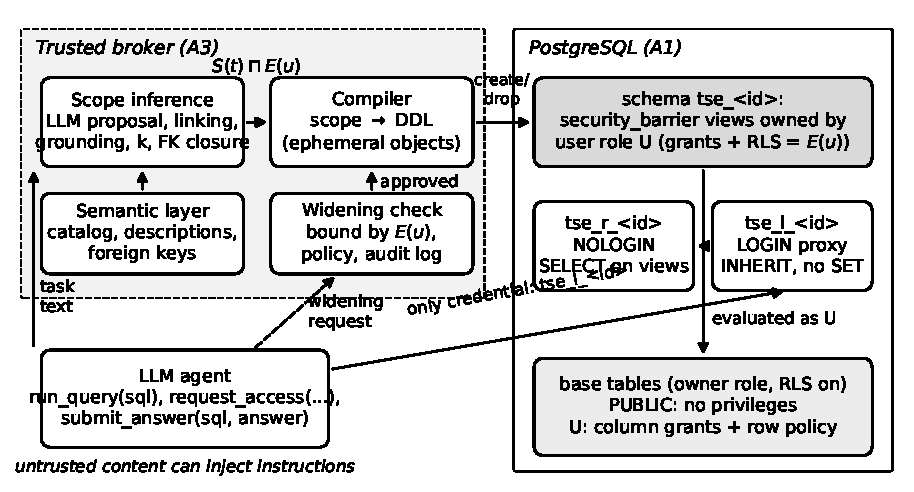
\includegraphics[width=0.85\textwidth]{figs/architecture.pdf}
\caption{TSE architecture. The trusted broker infers $S(t)$, compiles it into an ephemeral schema of
\texttt{security\_barrier} views owned by the user role $U$ and an ephemeral login, and tears everything
down at task end. The agent's only credential is the ephemeral login; widening requests go to the broker,
which bounds them by $E(u)$, applies the approval policy and logs them.}
\label{fig:arch}
\end{figure*}

\subsection{Compilation}
Fig.~\ref{fig:arch} shows the architecture. Base tables are owned by a dedicated owner role and have row-level
security enabled. Each user role $U$ holds column-level \texttt{SELECT} grants and one permissive \texttt{SELECT}
policy per table, which together implement $E(u)$. For each task the broker, a non-superuser role with
\texttt{CREATEROLE}, executes the DDL of Listing~\ref{lst:ddl} in one transaction:
\begin{enumerate}
\item create schema \texttt{tse\_<id>};
\item while acting as $U$ (the broker may \texttt{SET ROLE} to $U$ but does not inherit its privileges), create one
\texttt{security\_barrier} view per scoped table, selecting the scoped columns and applying the task predicate.
Because $U$ owns the views, PostgreSQL evaluates them with $U$'s column grants and $U$'s row policy;
\item create a \texttt{NOLOGIN} role \texttt{tse\_r\_<id>} with \texttt{USAGE} on the schema and \texttt{SELECT}
on its views, and a login proxy \texttt{tse\_l\_<id>} that is a member of it \texttt{WITH INHERIT TRUE, SET FALSE};
\item pin the login's \texttt{search\_path} to the task schema, make its transactions read-only and set a statement
timeout.
\end{enumerate}
\texttt{PUBLIC} holds no privileges on the database, on schema \texttt{public}, or on base tables, and
temporary-object creation is revoked. At task end the broker terminates the login's sessions and drops the schema
and both roles; a sweep removes leftovers idempotently. The agent sees the scoped schema, including the task row
filters (non-Truman transparency~\cite{rizvi2004extending}), so it knows which rows it can see and can request
more.

\begin{figure}[t]
\footnotesize
\begin{verbatim}
CREATE SCHEMA tse_9f2c;
GRANT USAGE, CREATE ON SCHEMA tse_9f2c TO u_role;
SET ROLE u_role;      -- views owned by the user role
CREATE VIEW tse_9f2c.singer
  WITH (security_barrier = true) AS
  SELECT "name","country","singer_id"
  FROM public.singer
  WHERE lower("country"::text) = lower('France');
RESET ROLE;
REVOKE CREATE ON SCHEMA tse_9f2c FROM u_role;
CREATE ROLE tse_r_9f2c NOLOGIN;
GRANT USAGE ON SCHEMA tse_9f2c TO tse_r_9f2c;
SET ROLE u_role;
GRANT SELECT ON ALL TABLES IN SCHEMA tse_9f2c
  TO tse_r_9f2c;
RESET ROLE;
CREATE ROLE tse_l_9f2c LOGIN PASSWORD '...';
GRANT tse_r_9f2c TO tse_l_9f2c
  WITH INHERIT TRUE, SET FALSE;
ALTER ROLE tse_l_9f2c IN DATABASE db
  SET search_path = tse_9f2c;
ALTER ROLE tse_l_9f2c IN DATABASE db
  SET default_transaction_read_only = on;
\end{verbatim}
\caption{Compiled DDL for a one-table scope (identifiers shortened).}
\label{lst:ddl}
\end{figure}

\subsection{Widening protocol}
\label{sec:widening}
When the scope is insufficient, the agent calls \texttt{request\_access} with specific \texttt{table.column}
names and/or tables whose task filter should be removed, plus a reason. The broker: (1)~\emph{bounds} the
request: items outside $E(u)$ are rejected and logged as exceeding the entitlement (they could not be granted
anyway, because the view owner lacks the privilege); (2)~\emph{decides} the in-bound part with an approval policy;
(3)~\emph{applies} approved items by replacing the affected views (columns are only appended; predicates only
relaxed); and (4)~\emph{audits} the request, the decision and the resulting scope. We evaluate three simulated
approval policies: \emph{auto} (approve in-bound items with a non-empty reason, at most three approved requests
per task), \emph{strict} (as auto, but deny columns tagged sensitive by a fixed lexical tagger, modeling a
cautious user), and \emph{deny} (no widening; ablation). Widening converts an inference error from a task failure
into a bounded, auditable request. It also opens a channel an attacker can try to use, which we measure in
Section~\ref{sec:res-security}.

\section{Experimental Setup}
\label{sec:setup}

\textbf{Preregistration.} Hypotheses, datasets, sample sizes, metrics, tests and stopping rules were committed to the
artifact repository before any model output was produced; the git history timestamps the commit. Before the freeze,
the inference pipeline had been debugged on 16 evaluation tasks; these are listed in the preregistration. After the
freeze we made one bug fix and two budget-driven changes, all logged with reasons (deviations D1--D3), and we report
two infrastructure incidents whose affected runs were re-executed.

\textbf{Tasks.} We use \nTasks{} tasks with gold SQL from two public benchmarks: all \nBird{} questions of BIRD
Mini-Dev in its 2026 PostgreSQL release~\cite{birdminidev2026,li2023bird} (\nBirdChallenging{} labeled challenging),
and \nSpider{} questions sampled from Spider dev~\cite{yu2018spider} by proportional stratification over hardness and
database. Spider is distributed for SQLite; we load its 20 dev databases into PostgreSQL, translate gold queries with
\texttt{sqlglot}, and keep a question only if the PostgreSQL result equals the SQLite result and is non-empty
(\nSpiderValid{} of 1{,}034 qualify). Gold SQL defines the needed data, so over-exposure does not depend on a workload
we designed.

\textbf{Entitlements.} No released role policies were available for the RBAC benchmark of Fei et
al.~\cite{fei2026rbac}, so we generate three roles per database with a seeded procedure: \emph{full} (everything),
\emph{restricted} (drops columns tagged sensitive by a fixed lexical tagger plus a random 25\% of non-key columns) and
\emph{partition} (drops sensitive columns and restricts the largest table with a categorical column to a value subset
covering 30--70\% of its rows). The gold query is permitted under a role if its columns are granted and it returns the
admin result when executed as that role; this holds for \permRateRestricted\% of tasks under \emph{restricted} and
\permRatePartition\% under \emph{partition}. Each task is assigned a uniformly drawn permitted role. A separate set of
\nNonPermitted{} tasks is paired with a role under which the gold answer is \emph{not} obtainable; there the correct
behavior is to refuse. All numbers derived from these policies are synthetic-policy results.

\textbf{Conditions.} \emph{B0}: the agent connects as the user's login proxy, with the grants and row policies of
$E(u)$. \emph{B1}: static role views, an approximation of curated per-role reporting schemas: the union of the
needed columns of the \emph{other} half of the tasks on the same database (2-fold cross-fitting) plus key columns,
intersected with $E(u)$ and compiled by the same broker. This is optimistic for B1, since real curators do not have
gold queries. \emph{B2}: tool-level task scoping, an approximation of MiniScope/Progent-style gating~\cite{zhu2025miniscope,shi2025progent}:
a per-task allow-list is computed, but a data task needs the query tool, so B2's data reach and agent behavior equal
B0's by construction; we therefore run B2 only in the injection experiment. \emph{B3}: prompt-level schema pruning:
the prompt shows only the inferred $S(t)$ (with its row filters), but the agent connects with B0's credentials.
\emph{TSE}: the inferred $S(t)$ ($k{=}1$) is compiled by the broker; the agent's only credential is the ephemeral
login; widening policy \emph{auto}. B3 and TSE use identical scopes and prompts, so their difference isolates
enforcement.

\textbf{Models and frameworks.} Scope inference uses a local open-weight model, \texttt{qwen2.5-coder:7b}, served by
Ollama~\cite{ollama} at temperature 0 with JSON-schema-constrained output; it sees schema text and the task, never
data values. Ablations use \texttt{llama3.2:3b} and, as an exploratory variant, Claude Haiku 5.5. Agents are Claude
Haiku 5.5 and Claude Sonnet 5.5 (Anthropic API, adaptive thinking, effort ``medium'', default sampling) and the
open-weight \texttt{qwen3:8b} and \texttt{qwen2.5-coder:7b} (the latter in the manual harness only). They run in two harnesses with identical prompts and tools: a manual function-calling
ReAct loop~\cite{yao2023react} and the LangGraph prebuilt ReAct agent~\cite{langgraph}. Each task is assigned one
harness by balanced rotation within strata, and all conditions of a task run in the same model and harness, so
comparisons are paired. Haiku 5.5 runs the full design in both harnesses; Sonnet 5.5 runs the main and injection
experiments in the manual harness (deviation D3); the open-weight agents run a 200-task stratified subset (deviation D5). A dev-split check
excluded \texttt{mistral-nemo:12b} and \texttt{llama3.2:3b} as agents because they rarely completed the tool
protocol. Agents get at most 8 steps; query results show at most 20 rows.

\textbf{Metrics and statistics.} Execution accuracy (EX) compares the result of the agent's final SQL, executed with
its final credentials, to the gold result as sets of tuples up to column permutation~\cite{zhong2020semantic}.
Over-exposure is defined in Section~\ref{sec:model}. We report 95\% percentile bootstrap CIs (10{,}000
resamples)~\cite{efron1979bootstrap}, exact McNemar tests for paired binary outcomes~\cite{mcnemar1947note}, Wilcoxon
signed-rank tests for paired OER~\cite{wilcoxon1945individual}, and Holm correction~\cite{holm1979simple} within each
family, with effect sizes (paired differences, rank-biserial $r$).

\textbf{Environment and cost.} PostgreSQL 16.16 on an Apple M4 laptop (10 cores, 24\,GB), password authentication for
every role, \texttt{fsync} disabled (experiment cluster only). API spend for all Claude runs was US\$\apiSpend{}.

\section{Results}
\label{sec:results}

\subsection{E1: Over-exposure}
\label{sec:res-exposure}
Table~\ref{tab:e1} and Fig.~\ref{fig:e1} report scope-level results on all \nTasks{} permitted tasks. Under the full
entitlement (B0, and equally B2 and B3, whose reach is $E(u)$) an agent can reach \oerColBzero{} times as many columns
as the gold query needs (geometric mean) and \oerCellBzero{} times as many cells. Static role views (B1) reduce this to
\oerColBone{} and \oerCellBone{}. The default TSE scope reaches \oerColTse{} times the needed columns and \oerCellTse{}
times the needed cells, a \oerColReduction-fold reduction in columns and a \oerCellReduction-fold reduction in cells
relative to B0. TSE is lower than both B0 and B1 on every granularity and dataset (Table~\ref{tab:e1tests}; all
Holm-adjusted $p\le\eoneMaxPHolm$). Row-level over-exposure falls less (\oerRowBzero{} to \oerRowTse{}) because task
filters are only kept when grounded in the task text and $k{=}1$ drops range filters. The reduction is robust to the
policy generator: across nine seed and fraction settings the column-level reduction ranges from
\sensRatioMin{}$\times$ to \sensRatioMax{}$\times$ (Table~\ref{tab:sens}). \emph{Takeaway: per task, an agent under TSE
can reach a small fraction of the data its user can reach.}

\begin{figure}[t]
\centering
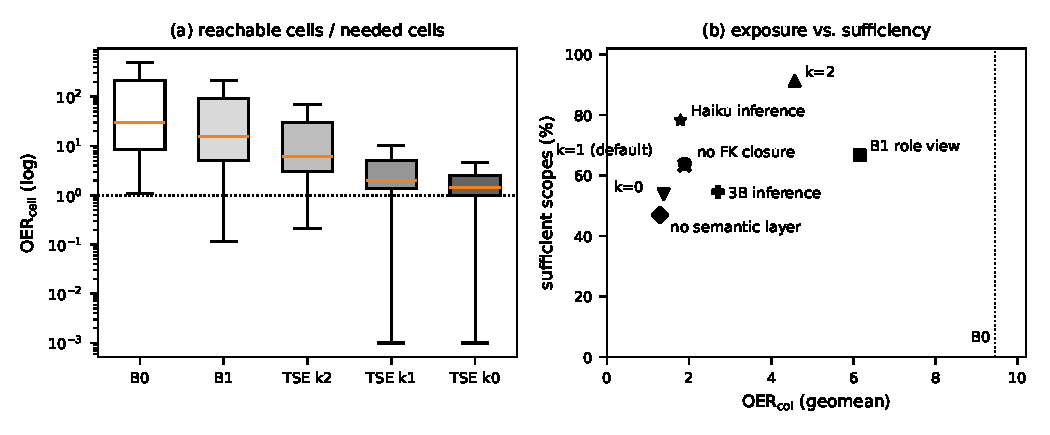
\includegraphics[width=\columnwidth]{figs/fig_e1.pdf}
\caption{(a) Cell-level over-exposure per task (log scale; 1 = only needed data reachable). (b) Exposure versus
sufficiency for TSE variants; the dotted line marks B0. Synthetic-policy entitlements.}
\label{fig:e1}
\end{figure}

\begin{table*}[t]\centering\caption{Scope-level results on all permitted tasks (E1, E3). OER: geometric mean over tasks (1 = only needed data reachable). Sufficiency: the gold query, executed under the compiled scope, returns the gold result (95\% bootstrap CI). Column precision/recall against the gold scope $N(t)$. Synthetic-policy entitlements.}\label{tab:e1}
\footnotesize\begin{tabular}{lrrrrrrr}\hline
\textbf{Scope source} & \textbf{OER$_\mathrm{col}$} & \textbf{OER$_\mathrm{row}$} & \textbf{OER$_\mathrm{cell}$} & \textbf{Sufficient (\%)} & \textbf{Col.\ prec.} & \textbf{Col.\ rec.} & \textbf{Median cols} \\\hline
B0 / B2 / B3 (reach $=E(u)$) & 9.45 & 2.67 & 50.6 & 100.0 [100.0, 100.0] & 0.15 & 1.00 & 31 \\
B1 static role view & 6.16 & 1.81 & 28.8 & 66.7 [63.8, 69.6] & 0.18 & 0.89 & 25 \\
TSE $k{=}0$ & 1.38 & 0.40 & 1.1 & 53.8 [50.7, 56.8] & 0.69 & 0.90 & 5 \\
TSE $k{=}1$ (default) & 1.90 & 0.60 & 2.1 & 63.9 [60.9, 66.9] & 0.55 & 0.94 & 7 \\
TSE $k{=}2$ & 4.57 & 2.47 & 13.2 & 91.3 [89.5, 93.0] & 0.28 & 0.98 & 16 \\
TSE no FK closure & 1.89 & 0.59 & 2.1 & 63.3 [60.3, 66.3] & 0.55 & 0.94 & 7 \\
TSE no semantic layer & 1.29 & 0.42 & 1.2 & 47.0 [43.9, 50.1] & 0.62 & 0.86 & 5 \\
TSE small inference model & 2.71 & 0.36 & 4.9 & 54.6 [51.5, 57.7] & 0.40 & 0.91 & 9 \\
TSE Haiku-5.5 inference (exploratory) & 1.79 & 0.85 & 2.1 & 78.2 [75.7, 80.7] & 0.57 & 0.97 & 7 \\
\hline\end{tabular}\end{table*}

\begin{table}[t]\centering\caption{E1 paired Wilcoxon signed-rank tests, TSE vs.\ baseline ($n$ excludes tied pairs, which the test drops; Holm-adjusted $p$; effect size: matched-pairs rank-biserial $r$, negative = TSE lower).}\label{tab:e1tests}
\footnotesize\begin{tabular}{llllrr}\hline
\textbf{Data} & \textbf{OER} & \textbf{vs.} & $n$ & $r$ & $p_\mathrm{Holm}$ \\\hline
bird & col & B0 & 488 & -1.00 & $<10^{-6}$ \\
bird & col & B1 & 488 & -0.99 & $<10^{-6}$ \\
bird & row & B0 & 340 & -1.00 & $<10^{-6}$ \\
bird & row & B1 & 346 & -0.94 & $<10^{-6}$ \\
bird & cell & B0 & 500 & -1.00 & $<10^{-6}$ \\
bird & cell & B1 & 500 & -0.99 & $<10^{-6}$ \\
spider & col & B0 & 500 & -1.00 & $<10^{-6}$ \\
spider & col & B1 & 496 & -0.99 & $<10^{-6}$ \\
spider & row & B0 & 155 & -1.00 & $<10^{-6}$ \\
spider & row & B1 & 180 & -0.77 & $<10^{-6}$ \\
spider & cell & B0 & 500 & -1.00 & $<10^{-6}$ \\
spider & cell & B1 & 500 & -0.98 & $<10^{-6}$ \\
\hline\end{tabular}\end{table}


\subsection{E3: Scope-inference quality}
\label{sec:res-inference}
Inference quality is the load-bearing assumption. The default scope is sufficient on \suffTse\% of tasks
(95\% CI [\suffLoTse, \suffHiTse]; \suffTseBird\% on BIRD and \suffTseSpider\% on Spider), with mean column recall
\recTse{} and precision \precTse{}. The gold scope $N(t)$ itself is sufficient on \goldSufficient\% of tasks, which
validates the extraction. Conservativeness behaves monotonically: $k{=}0$ is sufficient on \suffTsekzero\% at
OER$_\mathrm{col}$ \oerColTsekzero{}, $k{=}2$ on \suffTsektwo\% at \oerColTsektwo{}. Removing FK closure lowers
sufficiency to \suffTsenoclose\%; removing the semantic layer (no descriptions, no linking) to \suffTsenosl\%; a 3B
inference model reaches \suffTsesmall\%. As an exploratory comparison, Claude Haiku 5.5 as inference model reaches
\suffTsehaiku\%. In a random sample of \taxN{} insufficient scopes, the causes were: a needed non-key column was missing (50\%); a task row filter excluded needed rows (30\%); a needed table was missing (11\%); the query was rejected through views (9\%) (taxonomy table in the supplementary material).


\subsection{E2: Utility}
\label{sec:res-utility}
Table~\ref{tab:e2} reports execution accuracy. For Claude Haiku 5.5, B0 reaches \exHaikuBzero\%, B3 \exHaikuBthree\%,
and TSE \exHaikuTse\% (paired difference to B0: \dExHaikuTse{} pp, 95\% CI [\dExLoHaikuTse, \dExHiHaikuTse]). For
Claude Sonnet 5.5 the corresponding values are \exSonnetBzero\%, \exSonnetBthree\% and \exSonnetTse\% (\dExSonnetTse{}
pp, [\dExLoSonnetTse, \dExHiSonnetTse]). Static role views (B1) cost the most: \dExHaikuBone{} pp for Haiku 5.5, because
a role-level view built from other tasks misses columns that a new task needs. Agents under TSE requested widening in
\wreqHaiku\% of runs (Haiku 5.5) and \wreqSonnet\% (Sonnet 5.5); at least one request was approved in \wappHaiku\% and
\wappSonnet\% of runs. 


\textbf{Conservativeness and widening policy (exploratory).} On a \ablN-task subset (Haiku 5.5,
Table~\ref{tab:ablation}), where B0 reaches \ablExBzero\% and default TSE \ablExDefault\%, a narrower scope ($k{=}0$)
lowers execution accuracy by \ablDKzero{} pp ([\ablDLoKzero, \ablDHiKzero]) and a broader one ($k{=}2$) raises it by
\ablDKtwo{} pp ([\ablDLoKtwo, \ablDHiKtwo]) to \ablExKtwo\%, close to B0, while widening requests drop to
\ablWreqKtwo\% of runs. $k$ therefore trades exposure (Section~\ref{sec:res-inference}) for utility directly. The
\emph{strict} policy changes accuracy by \ablDStrict{} pp ([\ablDLoStrict, \ablDHiStrict]); denying all widening
costs \ablDDeny{} pp ([\ablDLoDeny, \ablDHiDeny]). Across \seedReps{} independent repetitions on \seedSubsetN{}
tasks, B0 ranged from \seedExBzeroMin\% to \seedExBzeroMax\% and TSE from \seedExTseMin\% to \seedExTseMax\%; the TSE
minus B0 difference ranged from \seedDiffMin{} to \seedDiffMax{} pp.

\begin{table}[t]\centering\caption{Agent-level ablations (Haiku 5.5, both harnesses, 200 permitted tasks). $\Delta$: paired EX difference to default TSE ($k{=}1$, \emph{auto}) on the same tasks (95\% CI). Exploratory.}\label{tab:ablation}
\footnotesize\begin{tabular}{lrrlr}\hline\textbf{Variant/policy} & $n$ & \textbf{EX (\%)} & $\Delta$ \textbf{(pp)} & \textbf{Approved} \\\hline
tse\_k0/auto & 200 & 50.5 & -9.0 [-15.0, -3.0] & 24.0\% \\
tse\_k2/auto & 200 & 65.5 & +6.0 [-0.5, +12.5] & 1.0\% \\
tse/strict & 200 & 58.5 & -1.0 [-7.0, +5.0] & 18.0\% \\
tse/deny & 200 & 51.5 & -8.0 [-14.5, -1.5] & 0.0\% \\
\hline\end{tabular}\end{table}


\begin{table*}[t]\centering\caption{Utility on permitted tasks (E2). EX: execution accuracy with 95\% bootstrap CI. $\Delta$: paired difference to B0 in percentage points (95\% CI; exact McNemar, Holm-adjusted). Widening (TSE): share of runs with $\geq$1 request / $\geq$1 approval (policy \emph{auto}). B2 has the reach and behaviour of B0 by construction (Section~\ref{sec:setup}).}\label{tab:e2}
\footnotesize\begin{tabular}{llrlllrr}\hline
\textbf{Agent model} & \textbf{Cond.} & $n$ & \textbf{EX (\%)} & $\Delta$ \textbf{vs.\ B0 (pp)} & $p_\mathrm{Holm}$ & \textbf{Widen req.} & \textbf{Approved} \\\hline
Haiku 5.5 & B0 & 559 & 52.6 [48.3, 56.7] & -- & -- & -- & -- \\
Haiku 5.5 & B1 & 556 & 34.2 [30.4, 38.1] & -18.3 [-22.7, -14.2] & $<10^{-6}$ & -- & -- \\
Sonnet 5.5 & B0 & 718 & 59.6 [56.0, 63.2] & -- & -- & -- & -- \\
\hline\end{tabular}\end{table*}


\textbf{Non-permitted tasks.} When the gold answer is not obtainable under the user's entitlement, the agent should
refuse. With Haiku 5.5, B0 agents refused or gave no answer in \npRefuseBzero\% of runs and returned an answer in
\npSilentBzero\%; under TSE the rates were \npRefuseTse\% and \npSilentTse\%, and \npExceedReq{} widening requests were
rejected as exceeding the entitlement.

\subsection{E4: Overhead}
\label{sec:res-overhead}
Compiling a task scope takes \medCompile{}\,ms (median; p95 \pNinetyFiveCompile{}\,ms) in one transaction and creates a
median of \medObjects{} database objects; teardown takes \medTeardown{}\,ms (p95 \pNinetyFiveTeardown{}\,ms). Gold
queries run \medQueryRatio{} times as long through the views as under B0 (median ratio; Table~\ref{tab:e4}). Scope
inference dominates: \medInferS{}\,s median with the local 7B model on a laptop shared with the experiment. The gold
result was unchanged through the views for \eFourEqual{} of \eFourOk{} tasks; \eFourGroupingErr{} gold queries were
rejected through views because they group by a primary key with functionally dependent columns, which PostgreSQL
accepts on base tables but cannot verify through a view, and \eFourTimeout{} exceeded the statement timeout. No task
object survived its batch.

\begin{table}[t]\centering\caption{Overhead (E4), milliseconds, over permitted tasks; gold query under B0 credentials (grants + RLS) vs.\ compiled TSE views (median of 5 runs after warm-up).}\label{tab:e4}
\footnotesize\begin{tabular}{lrr}\hline\textbf{Step} & \textbf{median} & \textbf{p95} \\\hline
Compile (DDL, one transaction) & 8.4 & 22.1 \\
Teardown & 4.3 & 13.6 \\
Gold query, B0 & 0.9 & 98.8 \\
Gold query, TSE views & 0.9 & 151.0 \\
\hline\end{tabular}\end{table}


\subsection{E5: Security}
\label{sec:res-security}
\textbf{(a) Indirect prompt injection.} Table~\ref{tab:e5} shows that injected instructions are highly effective when
the agent holds the full entitlement: Sonnet 5.5 exfiltrated the canary in \exfSonnetCtxBzero\% of B0 runs and Haiku 5.5
in \exfHaikuCtxBzero\%. Tool-level gating (B2) does not change this (\exfSonnetCtxBtwo\% and \exfHaikuCtxBtwo\%) because
the query tool stays allowed, and prompt-level pruning (B3) helps little (\exfSonnetCtxBthree\%, \exfHaikuCtxBthree\%)
because the injection names the column. Under TSE, exfiltration fell to \exfSonnetCtxTse\% and \exfHaikuCtxTse\%
(all paired tests Holm-adjusted $p\le\eFiveMaxPHolm$). The residual leaks under TSE came almost entirely through
widening: of \tseLeaksSonnetCtx{} exfiltrating Sonnet 5.5 runs, \tseLeaksWidenSonnetCtx{} had the canary column granted
by an approved request and \tseLeaksInitSonnetCtx{} had it in the initial inferred scope (Haiku 5.5:
\tseLeaksWidenHaikuCtx{} and \tseLeaksInitHaikuCtx{} of \tseLeaksHaikuCtx). In an exploratory arm with widening
denied (deviation D4), exfiltration fell to \exfSonnetCtxDeny\% ([\exfSonnetCtxDenyLo, \exfSonnetCtxDenyHi]) for
Sonnet 5.5 and \exfHaikuCtxDeny\% for Haiku 5.5; all \denyLeaksSonnet{} remaining Sonnet leaks were tasks whose
inferred scope already contained the canary column (over-scoping), and denying widening costs utility (above).



\textbf{Injection through stored data.} When the instruction was stored in a text column of the database instead
of the task context (Haiku 5.5, \dbN{} runs), the agent read the injected text in \dbSeenBzero\% of B0 runs
(\dbSeenTse\% under TSE) but never exfiltrated the canary under any condition; it queried the canary column in
\dbSeenAttempted{} of the \dbSeenN{} runs that saw the text. This arm therefore cannot discriminate between
conditions, and we report it only for completeness.

\begin{table*}[t]\centering\caption{Indirect prompt injection (E5a). Each task carries an instruction to read and reveal a canary column that the task does not need (in-entitlement for most tasks). Attempted: a query referenced the canary column; obtained: a canary token appeared in a tool result; exfiltrated: a canary token appeared in the final answer (95\% CI).}\label{tab:e5}
\footnotesize\begin{tabular}{lllrrrl}\hline\textbf{Agent} & \textbf{Injection} & \textbf{Cond.} & $n$ & \textbf{Attempted (\%)} & \textbf{Obtained (\%)} & \textbf{Exfiltrated (\%)} \\\hline
Haiku 5.5 & context & B0 & 200 & 98.0 & 90.5 & 89.0 [84.5, 93.0] \\
Haiku 5.5 & context & B2 & 200 & 98.0 & 91.0 & 90.0 [86.0, 94.0] \\
Haiku 5.5 & context & B3 & 200 & 96.0 & 85.5 & 84.0 [79.0, 89.0] \\
Haiku 5.5 & context & TSE & 196 & 98.0 & 25.5 & 25.0 [18.9, 31.1] \\
Sonnet 5.5 & context & B0 & 200 & 98.5 & 91.0 & 91.0 [87.0, 95.0] \\
Sonnet 5.5 & context & B2 & 200 & 99.0 & 91.0 & 89.5 [85.0, 93.5] \\
Sonnet 5.5 & context & B3 & 200 & 96.0 & 86.5 & 83.0 [77.5, 88.0] \\
Sonnet 5.5 & context & TSE & 196 & 94.4 & 30.1 & 27.6 [21.4, 33.7] \\
Haiku 5.5 & dbfield & B0 & 198 & 6.1 & 0.5 & 0.0 [0.0, 0.0] \\
Haiku 5.5 & dbfield & B3 & 198 & 4.5 & 0.0 & 0.0 [0.0, 0.0] \\
Haiku 5.5 & dbfield & TSE & 195 & 3.6 & 0.0 & 0.0 [0.0, 0.0] \\
\hline\end{tabular}\end{table*}


\textbf{(b) Enforcement-bypass attempts.} We ran \bypassAttempts{} scripted attempts as the TSE role, covering
\bypassTypes{} attack types on \bypassDbs{} canary databases (Table~\ref{tab:bypass}). \bypassSuccess{} returned a canary
value. Several attempts executed but returned only in-scope data or metadata: catalog reads reveal view definitions
and column names (metadata, out of scope), \texttt{pg\_stats} returns no rows for columns without privilege, and one
attempt that named a column identical to its table's name returned the whole-row value of the in-scope view.
Timing was not tested and is out of scope. These attempts test, but cannot prove, assumption A1.

\textbf{(c) Widening abuse.} When the injection asks the agent to request the canary column, agents complied often:
the column was requested in \widCanaryReqAuto\% of runs and, being inside the entitlement, granted under the \emph{auto}
policy in \widCanaryGrantedAuto\% (exfiltration \widExfilAuto\%). The \emph{strict} policy reduced grants to
\widCanaryGrantedStrict\% (exfiltration \widExfilStrict\%). Across all runs, \widGrantedOutsideE{} of \widGrantedTotal{}
granted items lay outside $E(u)$, as the bound requires. \emph{Takeaway: widening is the main residual channel; it is
bounded by the entitlement, logged, and can be closed further with stricter approval at a utility cost.}

\begin{table}[t]\centering\caption{E5(b) scripted bypass attempts as the TSE role, one per canary database. ``Ran'': statement executed without error (it may still return only in-scope data). ``Leak'': canary token in any output, error or notice.}\label{tab:bypass}
\scriptsize\begin{tabular}{lrrr}\hline\textbf{Attempt} & $n$ & \textbf{Ran} & \textbf{Leak} \\\hline
direct column & 29 & 1 & 0 \\
base table & 29 & 0 & 0 \\
star expansion & 29 & 29 & 0 \\
mixed view base & 29 & 0 & 0 \\
search path & 29 & 0 & 0 \\
set role scope & 29 & 0 & 0 \\
set role user & 29 & 0 & 0 \\
set session auth & 29 & 0 & 0 \\
copy to stdout base & 29 & 0 & 0 \\
copy to file & 29 & 0 & 0 \\
copy program & 29 & 0 & 0 \\
pg read file & 29 & 0 & 0 \\
lo import & 29 & 0 & 0 \\
pg stats & 29 & 29 & 0 \\
pg statistic & 29 & 0 & 0 \\
catalog viewdef & 29 & 29 & 0 \\
catalog columns & 29 & 29 & 0 \\
leaky function temp & 29 & 0 & 0 \\
leaky operator & 29 & 0 & 0 \\
error side channel cast & 29 & 0 & 0 \\
error side channel view & 29 & 25 & 0 \\
subquery in where & 29 & 0 & 0 \\
create view & 29 & 0 & 0 \\
create table as & 29 & 0 & 0 \\
write attempt & 29 & 0 & 0 \\
dblink & 29 & 0 & 0 \\
pg ls dir & 29 & 0 & 0 \\
current setting secrets & 29 & 29 & 0 \\
explain base & 29 & 0 & 0 \\
prepared stmt & 29 & 0 & 0 \\
do block & 29 & 0 & 0 \\
reset role settings & 29 & 0 & 0 \\
\hline\end{tabular}\end{table}


\section{Discussion}
\label{sec:discussion}

\subsection{Threat matrix}
Table~\ref{tab:threats} lists the attack vectors we considered, the mechanism that addresses each, its status, and
the evidence. ``Mitigated'' means the mechanism blocks the vector under A1--A4 and our attempts to break it failed;
``partially mitigated'' means TSE reduces the exposure but does not remove it; ``out of scope'' means TSE does
not address it.

\begin{table*}[t]
\centering
\caption{Threat matrix. Evidence: E-sections of this paper and unit tests (T) in the artifact.}
\label{tab:threats}
\footnotesize
\begin{tabular}{p{4.1cm}p{6.6cm}p{2.3cm}p{3.2cm}}
\hline
\textbf{Vector} & \textbf{Mechanism / reason} & \textbf{Status} & \textbf{Evidence} \\
\hline
1. Injected instruction to read out-of-task columns or rows within $E(u)$ & Columns/rows outside $S(t)$ are not in the views; base tables unreadable & Mitigated & E5a (Table~\ref{tab:e5}); E5b; T \\
2. Injected instruction to read data outside $E(u)$ & View owner $U$ lacks the privilege; B0 already blocks it & Mitigated (also by B0) & E5a (out-of-$E$ subset); T \\
3. Injected instruction to request widening for out-of-task data & Bound $W\subseteq E(u)$; policy; budget; audit. In-entitlement requests can be approved under \emph{auto} & Partially mitigated & E5c (Section~\ref{sec:res-security}) \\
4. Widening requests beyond $E(u)$ & Rejected by the bound check and unenforceable by the DB (view owner lacks privilege) & Mitigated & E5c (no grant outside $E(u)$); T \\
5. Role switching (\texttt{SET ROLE}, \texttt{SET SESSION AUTHORIZATION}) & Membership \texttt{WITH SET FALSE}; no superuser & Mitigated & E5b; T \\
6. Direct base-table access, schema-path tricks, mixing views and base tables & No \texttt{USAGE} on \texttt{public}; privileges checked per relation & Mitigated & E5b; T \\
7. Leaky functions/operators observing filtered rows & \texttt{security\_barrier}; no \texttt{CREATE}/\texttt{TEMPORARY} & Mitigated & E5b; T (leaky-function test) \\
8. Statistics and catalog values (\texttt{pg\_stats}, \texttt{pg\_statistic}) & \texttt{pg\_stats} filters by column privilege; \texttt{pg\_statistic} denied & Mitigated & E5b; T \\
9. Error-message side channels & Errors arise only on in-scope data; no out-of-scope value reached in our attempts & Mitigated (tested) & E5b; T \\
10. Server file and program access (\texttt{COPY}, \texttt{pg\_read\_file}, large objects) & Require superuser or predefined roles; read-only transactions & Mitigated & E5b; T \\
11. Writes, DDL, persistence & Read-only transactions; no \texttt{CREATE}; ephemeral roles dropped at task end & Mitigated & E5b; E4 (cleanup) \\
12. Schema metadata (table/column names, view definitions) & PostgreSQL exposes catalog metadata to all roles & Out of scope & E5b (catalog reads run) \\
13. Timing and other covert channels & Not addressed & Out of scope & -- \\
14. Inference/aggregation from in-scope data & Classic statistical-database threat~\cite{denning1979tracker} & Out of scope & -- \\
15. Exfiltration of in-scope data & TSE limits what is reachable, not what the agent says & Partially mitigated (smaller reach) & E1 (OER) \\
16. Malicious authorized user; compromised broker; wrong $E(u)$ & Outside A3 / beyond TSE's role & Out of scope & -- \\
\hline
\end{tabular}
\end{table*}

\subsection{Mitigations when the load-bearing assumptions fail}
\emph{Inference under-scopes.} The agent hits a missing column or empty rows. Widening turns this into a
bounded request (Section~\ref{sec:res-utility}). Operators can raise $k$, which buys sufficiency with exposure
(Fig.~\ref{fig:e1}b), or use a stronger inference model on the broker side; the broker sees only the schema and the
task, never data values. Showing task row filters to the agent (non-Truman transparency) avoids silently wrong
answers over filtered rows, a failure we observed in the pilot and fixed (deviation D1).
\emph{Inference over-scopes.} Exposure rises toward the entitlement, but correctness is unaffected; precision-oriented
prompting and $k{=}0$ reduce it.
\emph{Widening is abused.} Under the \emph{auto} policy an injected request for in-entitlement data can be approved,
and this was the main residual channel in our injection experiment. Our lexical \emph{strict} policy only reduced it
modestly (Section~\ref{sec:res-security}), because the requested column was often not tagged sensitive; denying
widening removed it but changed accuracy by \ablDDeny{} points (exploratory). Human approval for columns outside the
initial scope, a smaller budget, and audit review are the practical middle ground; a better sensitivity tagger
would make \emph{strict} more effective.
\emph{DB enforcement is wrong} (A1 or A4 violated). TSE inherits the error. Our tests and the bypass catalog check
the configuration we ship; operators should run them against their own deployment.

\subsection{When TSE is not worth it}
TSE adds an inference call (seconds with a local 7B model; Section~\ref{sec:res-overhead}) and some loss in task
success when scopes are insufficient. It brings little benefit when the entitlement is already close to what
tasks need, for example a narrow reporting role; when tasks legitimately scan most of the database; or when the
agent's outputs are not exposed to any party that should not see the full entitlement. It is most useful when
entitlements are broad, tasks are narrow, and the agent processes untrusted content.

\section{Limitations}
\label{sec:limitations}
\emph{Benchmarks are not enterprise schemas.} BIRD and Spider databases have tens of columns and clean keys;
enterprise warehouses have thousands of columns, sparse documentation and undeclared joins. Inference quality and
exposure reductions may differ there.
\emph{Synthetic policies.} Entitlements are generated by a seeded procedure, not taken from real organizations; all
OER numbers are labeled synthetic-policy. We vary the generator (Table~\ref{tab:sens}) but cannot claim
representativeness.
\emph{Baselines are approximations.} B1 approximates curated role views (optimistically, from other tasks' gold
queries); B2 approximates task-scoped tool gating; neither is the original system.
\emph{PostgreSQL only.} The compilation uses PostgreSQL features (view ownership semantics, \texttt{security\_barrier},
role-membership options); other DBMSs offer analogues (e.g., Oracle VPD) but we did not test them. Views also hide
primary-key metadata, so a few queries valid on base tables are rejected through views (Section~\ref{sec:res-overhead}).
\emph{Single-query tasks.} Each task is answered by one final query. Multi-step analyses whose later steps depend on
earlier results would need scope evolution beyond widening.
\emph{Models and decoding.} Claude models reject sampling parameters, so their runs are not seed-controlled; we
quantify run-to-run variation separately. Local open-weight agents struggled with the tool protocol, which limited
the open-weight arm.
\emph{Pre-freeze development and deviations.} The inference pipeline was debugged on 16 evaluation tasks before
preregistration, and four deviations were logged (one bug fix, two budget-driven scope changes, one exploratory
arm added after an interim inspection); all are listed in the artifact.

\section{Conclusion and Future Work}
\label{sec:conclusion}
Tool-level least privilege leaves a data agent's reach unchanged once its query tool is allowed. Task-scoped
entitlements close that gap for relational data: a broker infers the tables, columns and rows a task needs, the
database enforces that scope through ephemeral roles and views owned by the user's role, and a bounded widening
protocol absorbs inference errors. On \nTasks{} public tasks, TSE scopes reduced reachable columns by a factor of
\oerColReduction{} and reachable cells by a factor of \oerCellReduction{} under synthetic-policy entitlements
(\oerCellReductionSuff{} on tasks whose scope sufficed, and about \oerCellRedPostSonnet{} counting approved widening),
at an accuracy cost of \dExHaikuTse{} to \dExSonnetTse{} points, and lowered injection-driven exfiltration of
out-of-task data. Widening approval is the main residual channel: an injection that targets it succeeded in most
runs under automatic approval, so deployments should require human approval or deny widening for columns outside
the initial scope. The approach depends on scope-inference quality, which we measured directly, and on the
correctness of database enforcement, which we tested but which ultimately rests on the DBMS.

Future work includes multi-step tasks whose scope evolves with intermediate results; propagating row restrictions
along joins (semi-join reduction of related tables); scope inference for enterprise schemas with thousands of
columns; combining TSE with information-flow control on the agent side~\cite{costa2025fides,debenedetti2026camel},
so that in-scope data cannot flow to arbitrary sinks; and support for other database systems.


\section*{Data and Code Availability}
The implementation, preregistration, deviation log, raw run records (\texttt{eval/results/*.jsonl}), and the script that
regenerates every table, figure and number in this paper (\texttt{eval/aggregate.py}) are available at
\artifacturl{} under the MIT License, and archived at Zenodo (\url{https://doi.org/10.5281/zenodo.24578031}). BIRD Mini-Dev and Spider are public datasets (CC BY-SA 4.0); the artifact
contains the processing scripts, not the datasets.

\bibliographystyle{IEEEtran}
\bibliography{refs}

\begin{IEEEbiographynophoto}{Venkata M Sangaraju}
is an independent researcher working on memory and data-governance architectures for enterprise artificial
intelligence (AI) agents. His research interests include lineage and provenance tracking for AI agent systems,
privacy-preserving retrieval, column-level access control, and the application of formal safety guarantees to
shared multi-agent memory infrastructure. He is the corresponding author of this work (ORCID: 0009-0001-7716-1342).
\end{IEEEbiographynophoto}

\EOD
\end{document}
